\documentclass{extarticle} % Type du document
\usepackage[french]{babel} % Langue du document
\usepackage[T1]{fontenc}
\usepackage[utf8]{inputenc}
\usepackage[left=20mm, right=20mm, top=30mm, bottom=30mm]{geometry} % Définition de la largeur des marges gauches et droites
\usepackage{a4wide} % Format de la feuille
\usepackage{amsmath} % Pour inclure des équations
\usepackage{graphicx} % Pour inclure des images / graphiques
\usepackage{float} % Pour gérer le placement des images
\usepackage{fancyhdr} % Pour les headers, paramètres ci-dessous
\usepackage{tabularx}
\usepackage{array}
\usepackage{xcolor}
\usepackage{enumitem}
\usepackage{hyperref}
\usepackage{minted}
\usepackage{url}

\definecolor{lightgray}{rgb}{0.83, 0.83, 0.83}


\pagestyle{fancy}
\lhead{Nikolaos Garanis, Nathanaël Mizutani}
\rhead{SOS - Windows}
\cfoot{\thepage}

\title{SOS - Windows\\Laboratoire Password Theft et Persistence}
\author{Nikolaos Garanis, Nathanaël Mizutani}
\date{15.05.2019}

\begin{document}
    \maketitle

    \section{Reconnaissance}

    \subsection{Expliquer l'utilité de l'argument -Pn}
    Par défaut \texttt{nmap} va d'abord commencer par scanner le réseau à l'aide de pings pour découvrir les machines vivantes.
    Une fois celles-ci trouvées \texttt{nmap} va les sonder plus en profondeur selon ce qui aura été spécifié par l'utilisateur
    (scan de port, scan de services, ...).

    L'argument \texttt{-Pn} (No Ping) sert à sauter la phase de découverte des hôtes en les traitant tous comme étant en ligne.
    Il va ainsi effectuer les scans demandés sur toutes les machines du réseau.

    \subsection{Quel est le contrôleur de domaine ? Comment pouvez-vous le déterminer (2 façon distinctes)?}
    Le contrôleur de domaine est la machine dont l'IP est \texttt{172.22.4.2}.

    \begin{description}
        \item On peut déterminer quelle machine est le contrôleur de domaine :
    \end{description}
    \begin{enumerate}[label=>]
        \item en regardant quelle machine a les ports 53 (\texttt{domain}) et 88 (\texttt{kerberos-sec}) ouverts.
        \begin{figure}[H]
            \centering
            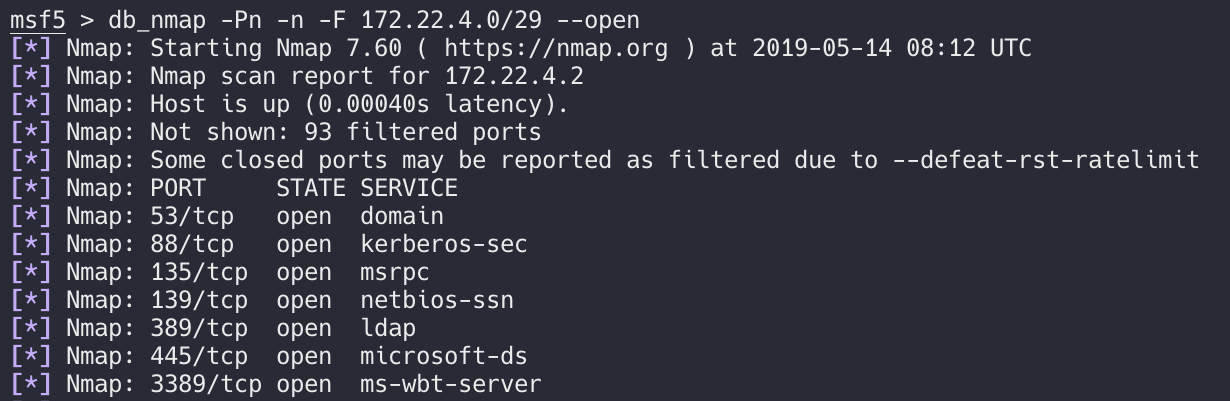
\includegraphics[scale=0.25]{images/port_scan.png}
            \caption{Résultat du scan de ports}
        \end{figure}
        \item en regardant le nom de la machine, ici \texttt{WAD-DC-SRV2} (avec DC : Domain Controller).
        \begin{figure}[H]
            \centering
            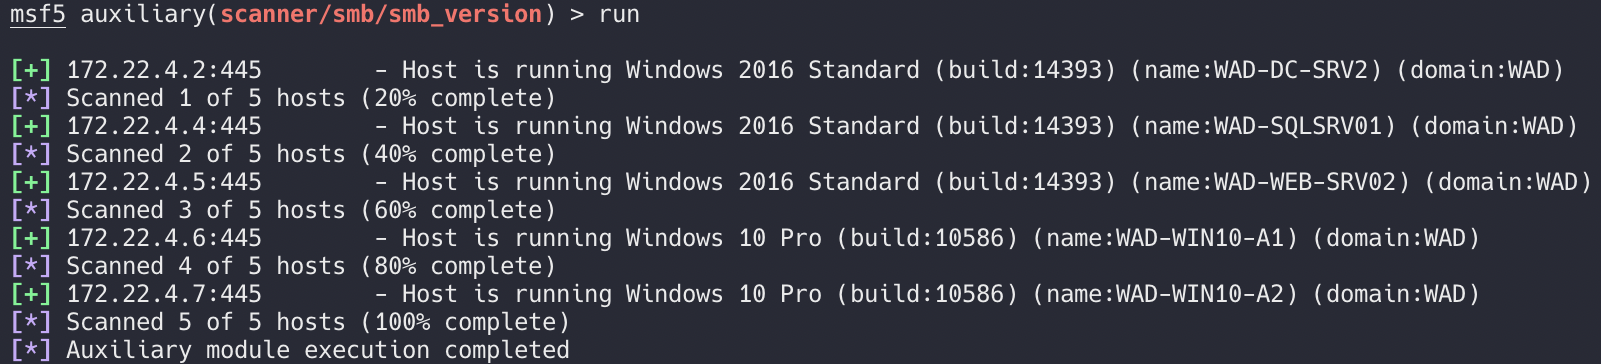
\includegraphics[scale=0.25]{images/smb_scan.png}
            \caption{Résultat du scan smb}
        \end{figure}
    \end{enumerate}

    \section{Exploitation de vulnérabilités logicielles}
    %LHOST: 172.22.3.151
    \subsection{Quels sont les droits d’exécution que vous obtenez ?}
    On obtient les droits d'exécution du compte \texttt{NT AUTHORITY\textbackslash SYSTEM}, lequel fait parti de \texttt{Builtin\textbackslash Administrator}.
    On a ainsi les droits administrateurs sur la machine.

    \subsection{Comment expliquer que vous disposez d’autant de privilège ?}
    On passe par un processus \texttt{smb} pour effectuer l'exploit, or ce processus possède des droits administrateurs. On hérite
    donc des droits \texttt{Administrator} de celui-ci.

    \subsection{Quel processus exécute votre \textit{meterpreter} sur la machine victime (identifiant et nom) ?}
    \texttt{meterpreter} exécute un \texttt{powershell} (pid 4012) sur la machine victime.

    \subsection{Quelle est la différence entre la version \textit{reverse\_tcp} et \textit{bind\_tcp} de \textit{meterpreter} ?}
    Avec la version \texttt{reverse\_tcp}, \texttt{meterpreter} demande à la machine victime de venir se connecter sur celle de l'attaquant.
    Tandis qu'avec \texttt{bind\_tcp}, c'est l'attaquant qui va se connecter à la machine victime.

    \subsection{Dans quelle situation est-il recommandé d’utiliser la version \textit{reverse\_tcp} ?}
    Si un pare-feu bloque les connexions entrantes mais pas les connexions sortantes, il est plus intéressant d'utiliser \texttt{reverse\_tcp}.

    \subsection{Dans la sortie de l’exécution, la notion de \textit{stage} apparaît, de quoi s’agit-il ?}
    Un \texttt{stage} est un composant téléchargé par le \textit{payload} pour lui ajouter des fonctionnalités.
    Contrairement à le \textit{payload}, les \textit{stages} n'ont pas de contraintes sur la taille.

    \section{Vol de credentials}

    \subsection{Décrivez la structure des entrées récupérées depuis la base SAM}
    On récupère les entrées de la base SAM avec la commande meterpreter \texttt{run post/windows/gather/hashdump}.
    La structure des entrées se présente comme suit :

    <Nom du compte>\textbf{:}<id du compte>\textbf{:}<hash LM>\textbf{:}<hash NTLM>\textbf{:::}

    \subsection{Comment expliquer que plusieurs comptes partagent les mêmes hashs ?}
    Parce que les mots de passe de ces comptes possèdent les mêmes 14 premiers caractères ou moins s'ils sont plus courts.

    \subsection{Est-ce que plusieurs machines utilisent les mêmes mots de passe locaux (utilisez \textit{smb\_login}) ?}
    Deux machines (172.22.4.6 et 172.22.4.7) utilisent les mêmes mots de passe pour l'utilisateur Administrator.

    \begin{figure}[H]
        \centering
        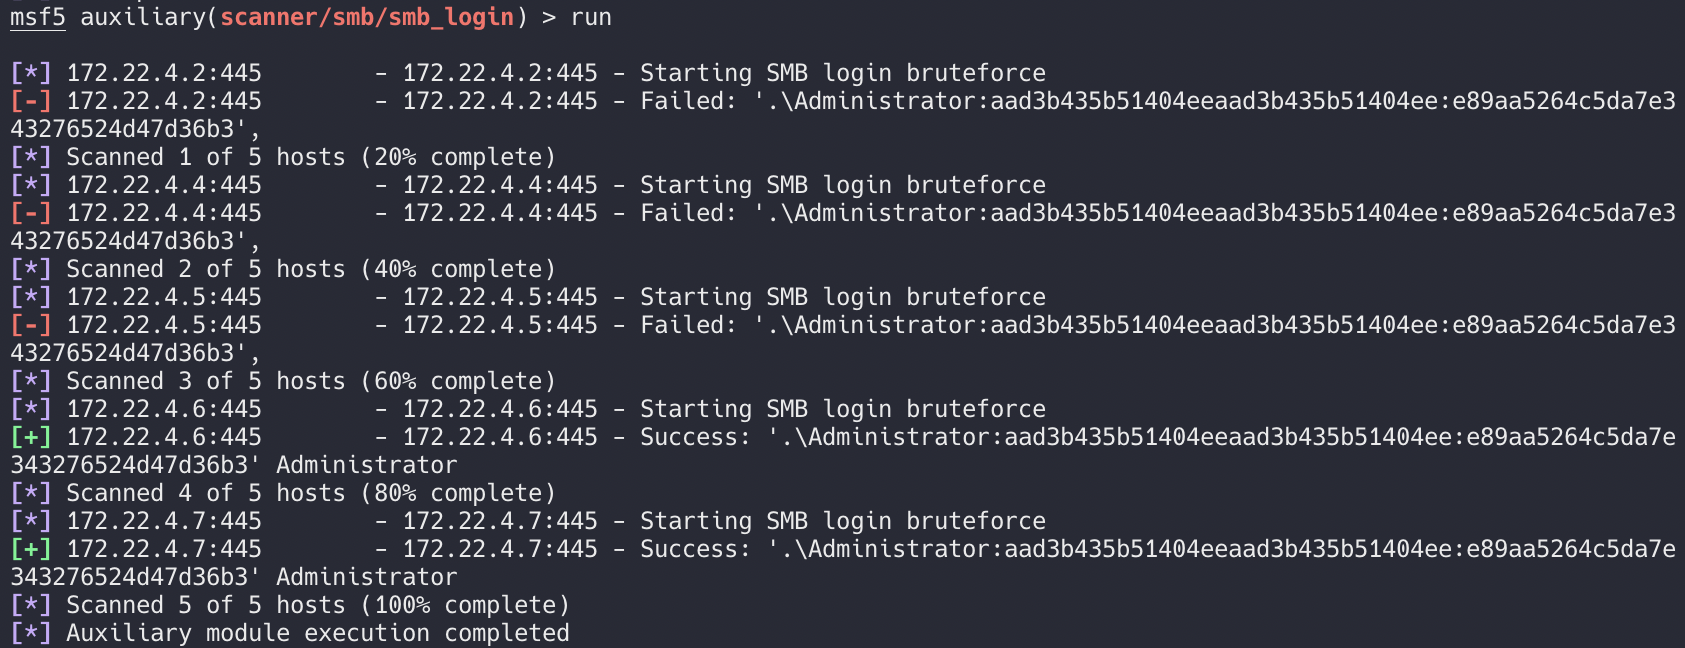
\includegraphics[scale=0.3]{images/same_pwd.png}
        \caption{Comptes avec le même mot de passe}
    \end{figure}

    \subsection{Quel est le format de hash utilisé pour stocker les hash MS-CACHE ? A quoi correspondent les
    différentes parties ?}
    Le format du hash MD4 est le suivant: \texttt{$MD4( MD4(Unicode(password)) + Unicode(tolower(username)) )$}.
    Il est composé des identifiants (nom d'utilisateur et mot de passe) de l'utilisateur.

    \subsection{À quoi correspond le compte qui se termine par un \$ retrouvé dans la mémoire de LSASS ?}
    Il s'agit d'un compte machine. Celui-ci est automatiquement créé lorsque la machine se connecte au domaine.
    Cependant nous n'en avons pas trouvé dans LSASS, mais en chargeant Mimikatz. Il s'agit du compte \texttt{WAD-SQLSRV01\$}.

    \subsection{Quel type de compte est nécessaire afin d’accéder au GPO sur le partage SYSVOL ?}
    Il faut un compte du domaine pour accéder au GPO sur le partage SYSVOL.

    \subsection{Quel est l’identifiant de la GPO qui contient le mot de passe ?}
    L'identifiant de la GPO est la \texttt{clsid} suivante : \texttt{CC63F200-7309-4ba0-B154-A71CD118DBCC}.

    \subsection{Quelle est la valeur chiffrée en CPassword qui correspond au mot de passe trouvé dans la GPP ?}
    La valeur du CPassword trouvé dans la GPP est \texttt{F7mL0Gt49wv64Y8HxukelyarUAwwd2BfPagryCKMRP8}.

    \begin{figure}[H]
        \centering
        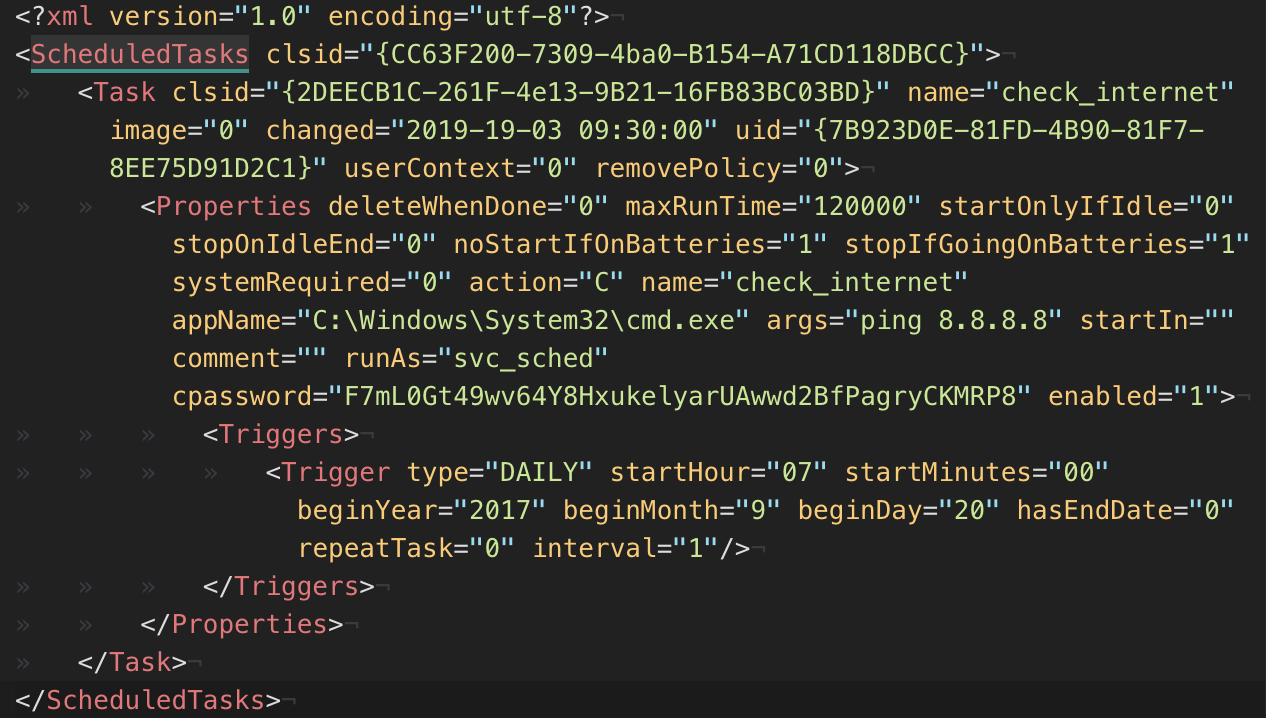
\includegraphics[scale=0.5]{images/cpassword.png}
        \caption{GPP}
    \end{figure}

    \subsection{Est-ce que ce compte est utilisé sur l’une des machines (\textit{smb\_login}) ?}
    Le compte local \texttt{svc\_sched} est utilisé seulement sur la machine 172.22.4.2 (contrôleur de domaine).

    \begin{figure}[H]
        \centering
        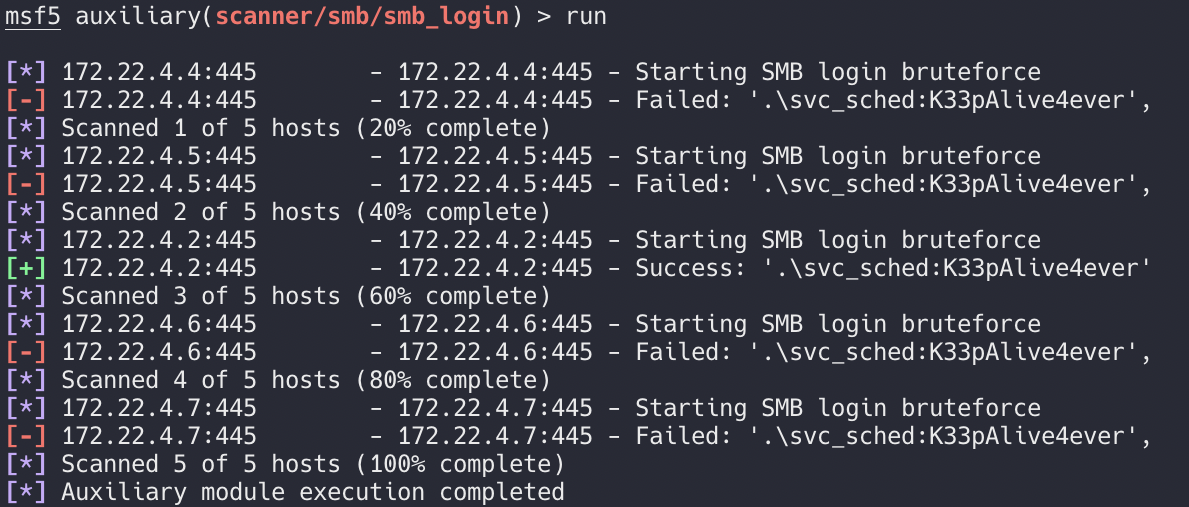
\includegraphics[scale=0.4]{images/p17.png}
        \caption{compte svc\_sched}
    \end{figure}

    \section{Kerberoast}

    \subsection{Expliquer pourquoi une seule entrée est retournée par le module ?}
    Le module cherche les SPN utilisés par des comptes utilisateurs dans le domaine spécifié. Une fois ces SPN trouvés, il soumet des requêtes
    pour obtenir des tickets TGS.

    Ainsi, seule une entrée est retournée car c'est le seul service vulnérable pour lequel le module a obtenu un ticket TGS.

    \subsection{Quel est le SPN complet vulnérable ?}
    Il s'agit de \texttt{MSSQLSvc/WAD-SQLSRV01.WAD.local:1433}.

    \begin{figure}[H]
        \centering
        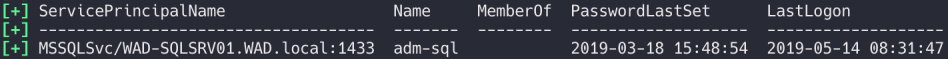
\includegraphics[scale=0.5]{images/SPN-vulnerable.png}
        \caption{SPN vulnérable}
    \end{figure}

    \subsection{Quel est le compte du domaine associé à ce SPN ?}
    Le compte associé à ce SPN est \texttt{adm-sql}.

    \subsection{Est-ce que ce compte est utilisé sur l’une des machines (utilisez \textit{smb\_login}) ?}
    Ce compte est utilisé sur les machines 172.22.4.2, 172.22.4.4, 172.22.4.5, 172.22.4.6, 172.22.4.7.
    Sur la machine 172.22.4.4, c'est un compte \texttt{Administrator}.

    \begin{figure}[H]
        \centering
        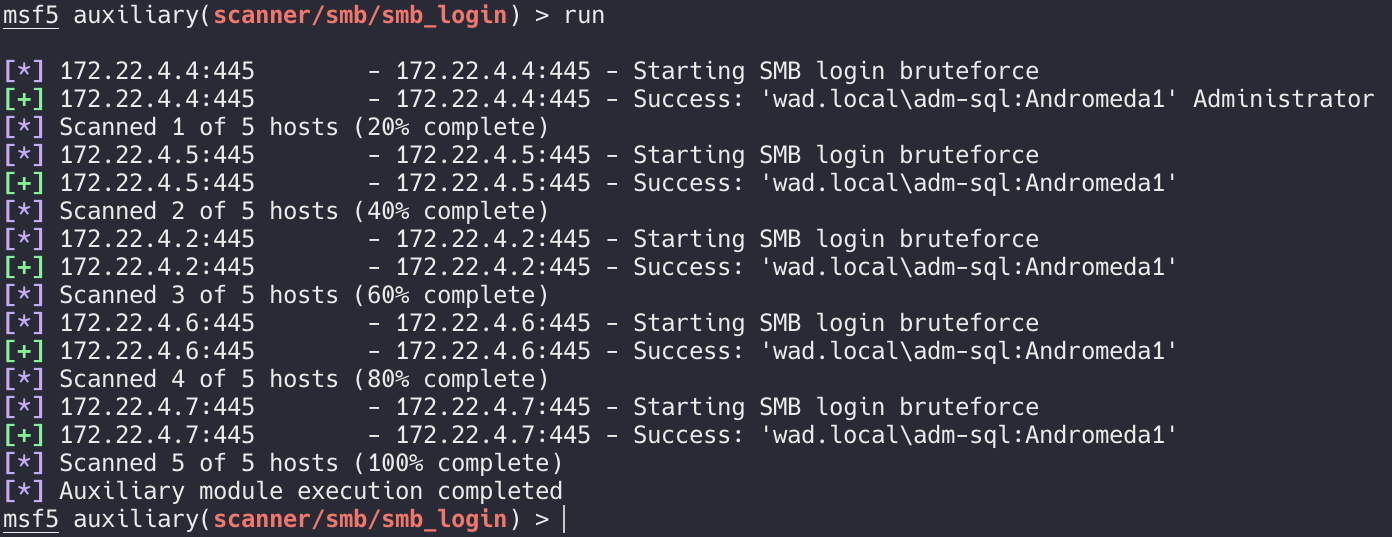
\includegraphics[scale=0.3]{images/adm-sql-admin-4.png}
        \caption{Compte Administrator sur 172.22.4.4}
    \end{figure}

    \subsection{Analyser les logs au moment de l’attaque et décrivez comment psexec fonctionne ?}
    Lorsq'on utilise \texttt{psexe} on obtient le log suivant :

    \begin{minted}[style=friendly, bgcolor=lightgray]{bash}
    [*] Started reverse TCP handler on 172.22.3.151:4444
    [*] 172.22.4.5:445 - Connecting to the server...
    [*] 172.22.4.5:445 - Authenticating to 172.22.4.5:445 as user 'Administrator'...
    [*] 172.22.4.5:445 - Selecting PowerShell target
    [*] 172.22.4.5:445 - Executing the payload...
    [+] 172.22.4.5:445 - Service start timed out, OK if running a command or non-service
    executable...
    [*] Sending stage (206403 bytes) to 172.22.4.5
    [*] Meterpreter session 8 opened (172.22.3.151:4444 -> 172.22.4.5:58477) at 2019-05-14
    17:15:33 +0000
    \end{minted}

    \texttt{psexe} se connecte à la machine distante puis ouvre dans celle-ci un powershell puis redirige le flux d'entrée
    vers la machine locale.

    \subsection{Quels sont les privilèges requis pour l’utilisation de psexec ?}
    On doit avoir les privilèges \texttt{Administrator} pour utiliser \texttt{psexe}. L'utilisation des PsTool demande d'être connecté
    au compte \texttt{ADMIN\$}.

    \subsection{Quelle vulnérabilité exploitez-vous pour rebondir sur le second serveur ?}
    Nous avons utilisé un \textit{Pass-the-hash} pour accéder au second serveur.

    \subsection{Comment avez-vous pu récupérer un compte du domaine sur le second serveur ?}
    Nous avons utilisé Mimikatz pour récupérer les identifiants de l'administrateur du domaine WAD-DC-SRV2 présents sur le serveur.
    On récupère ensuite le hash NTML de l'administrateur, puis on le concatène avec l'un des hash LM commun à tous les comptes.
    Avec ce hash reconstitué nous nous connectons au compte de l'administrateur du domaine.

    \begin{figure}[H]
        \centering
        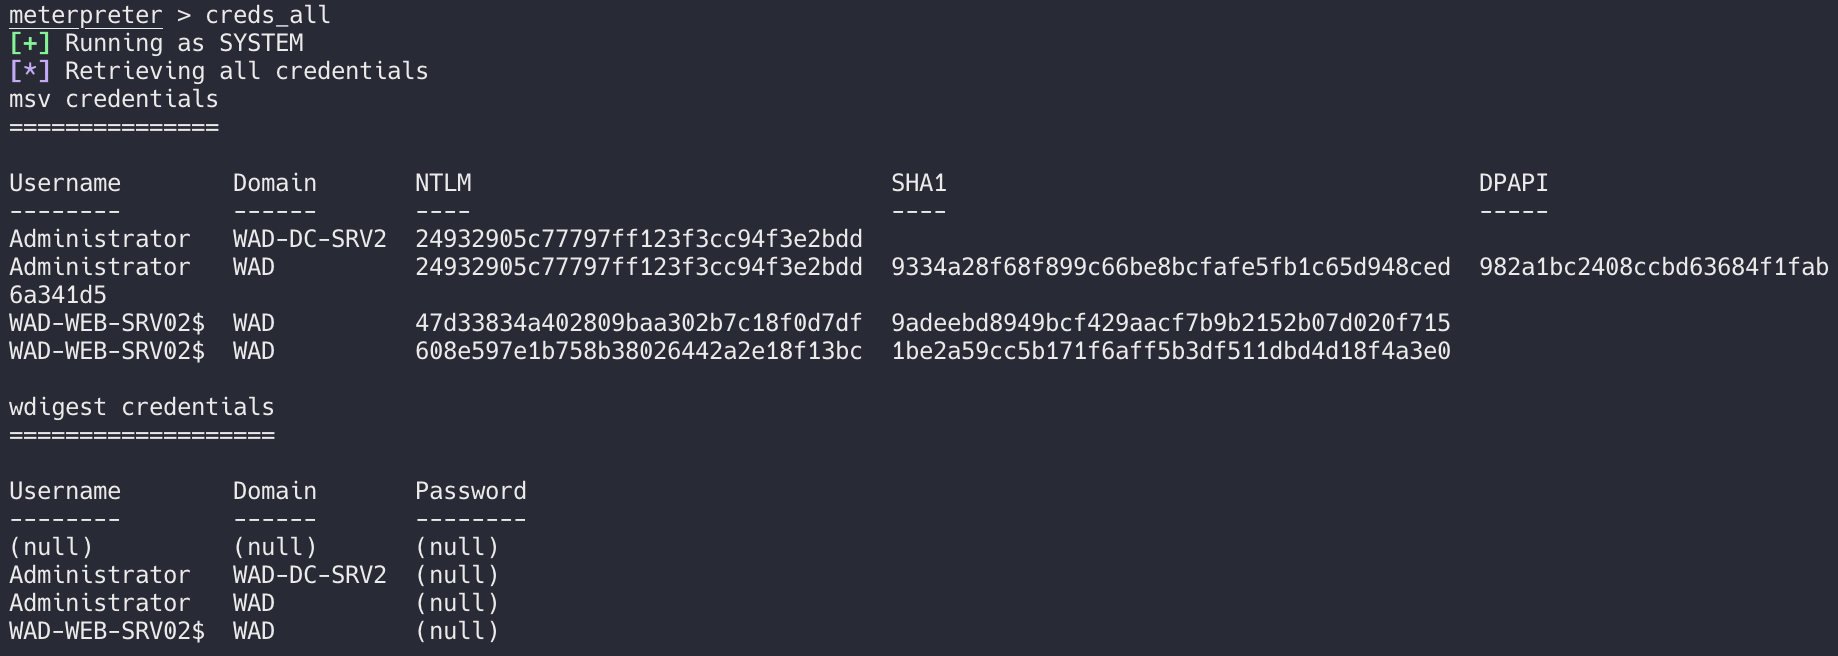
\includegraphics[scale=0.25]{images/creds-dc-srv.png}
        \caption{Hash NTLM de WAD-DC-SRV2}
    \end{figure}

    \subsection{Quelles sont les actions qui justifient l’utilisation d’un compte « Domain Admins » ?}
    Toutes les actions qui concernent directement l'administration du domaine. Par exemple, le déploiement d'un logiciel sur
    toutes les machines ou l'ajout d'une nouvelle machine au domaine.

    \subsection{Comment éviter qu’un de ces comptes puisse être volé ?}
    Pour éviter que l'un de ces comptes puisse être compromis, on change régulièrement son mot de passe.
    On s'assure aussi que les mots de passe soient suffisamment solides (complexité, longueur).
    À chaque fois qu'un administrateur se connecte sur une machine, il faut qu'il la redémarre en se déconnectant.

    \subsection{Qu’est-ce qui se passe quand vous essayez de monter le partage la première fois ?}
    Nous obtenons l'erreur « The password is invalid ».

    \begin{figure}[H]
        \centering
        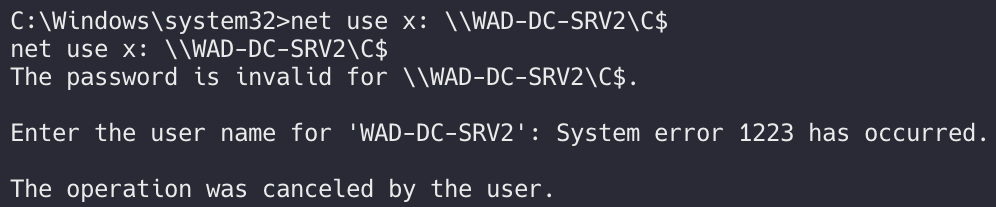
\includegraphics[scale=0.3]{images/c_dc_first_try.png}
        \caption{Première tentative}
    \end{figure}

    \subsection{Qu’est-ce qui se passe quand vous essayez de monter le partage la seconde fois ? Comment expliquer cette différence ?}
    La montage fonctionne la deuxième fois car nous avons les droits nécessaires. En effet, grâce au \textit{Golden Ticket} nous avons généré un ticket TGS
    nous donnant les droits administrateur.

    \begin{figure}[H]
        \centering
        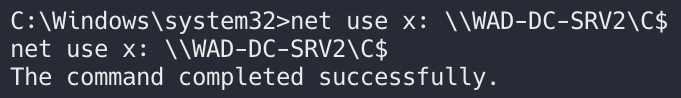
\includegraphics[scale=0.3]{images/c_dc_second_try.png}
        \caption{Deuxième tentative}
    \end{figure}

    \subsection{Localiser l’événement généré au moment de l’authentification avec le Golden Ticket dans les logs du DC}

    \begin{figure}[H]
        \centering
        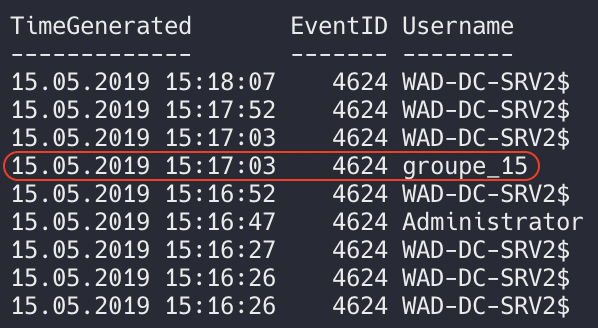
\includegraphics[scale=0.3]{images/gd_logs.png}
        \caption{Log lors de l'authentification avec le golden ticket}
    \end{figure}

    \subsection{Combien de temps est valable le golden ticket que vous avez généré ?}
    Par défaut un ticket kerberos dure 10 heures. Cependant le \textit{Golden Ticket} généré par Mimikatz est valable pour 10 ans et renouvelable.

    \subsection{Qu’est ce que l’administrateur du domaine doit faire s’il détecte qu’un attaquant a compromis le hash du compte krbtgt ?}
    Changer rapidement et deux fois de suite le mot de passe du compte krbtgt pour révoquer tous les tickets courants. Ensuite immédiatement
    contacter l'équipe de gestion des incidents.

    \pagebreak
    \section{Sources}
    \begin{enumerate}[label=$\bullet$]
        \item \url{https://buffered.io/posts/staged-vs-stageless-handlers/}
        \item \url{https://www.offensive-security.com/metasploit-unleashed/meterpreter-basics/}
        \item \url{https://security.stackexchange.com/questions/161889/understanding-windows-local-password-hashes-ntlm}
        \item \url{https://en.wikipedia.org/wiki/NT_LAN_Manager}
        \item \url{https://docs.microsoft.com/en-us/windows/security/threat-protection/security-policy-settings/maximum-lifetime-for-service-ticket}
        \item \url{https://security.stackexchange.com/questions/30889/cracking-ms-cache-v2-hashes-using-gpu}
        \item \url{https://www.helloitsliam.com/2016/02/10/understanding-metasploit-payloads/}
        \item \url{https://support.microsoft.com/en-us/help/253821/system-error-85-with-net-use-command}
        \item \url{http://rycon.hu/papers/goldenticket.html}
        \item \url{https://superuser.com/questions/265216/windows-account-ending-with}
        \item \url{https://pentestlab.blog/tag/service-principal-name/}
        \item \url{https://adsecurity.org/?p=1515}
        \item \url{https://github.com/rapid7/metasploit-framework/pull/9718/commits/8d12118d1f9333e92b0de7d7350a7f0b2ed1a4c6}
        \item \url{https://docs.microsoft.com/en-us/previous-versions/technet-magazine/cc162490(v=msdn.10)}
        \item \url{https://www.itprotoday.com/compute-engines/psexec}
    \end{enumerate}

\end{document}
